% Baseado em bare_conf.tex

\documentclass[conference]{IEEEtran}
\usepackage[utf8]{inputenc}
\usepackage[pdftex]{graphicx}
\usepackage{float}
\usepackage{color}
\IEEEoverridecommandlockouts



% *** SPECIALIZED LIST PACKAGES ***
%
%\usepackage{algorithmic}
% algorithmic.sty was written by Peter Williams and Rogerio Brito.
% This package provides an algorithmic environment fo describing algorithms.
% You can use the algorithmic environment in-text or within a figure
% environment to provide for a floating algorithm. Do NOT use the algorithm
% floating environment provided by algorithm.sty (by the same authors) or
% algorithm2e.sty (by Christophe Fiorio) as IEEE does not use dedicated
% algorithm float types and packages that provide these will not provide
% correct IEEE style captions. The latest version and documentation of
% algorithmic.sty can be obtained at:
% http://www.ctan.org/tex-archive/macros/latex/contrib/algorithms/
% There is also a support site at:
% http://algorithms.berlios.de/index.html
% Also of interest may be the (relatively newer and more customizable)
% algorithmicx.sty package by Szasz Janos:
% http://www.ctan.org/tex-archive/macros/latex/contrib/algorithmicx/

% correct bad hyphenation here
%\hyphenation{op-tical net-works semi-conduc-tor}


\begin{document}
\title{Trekking/Robo-Magellan Project}

\author{\IEEEauthorblockN{Tiago Koji Castro Shibata}
\IEEEauthorblockA{ThundeRatz Robotics Team\\
Escola Politécnica da\\
Universidade de São Paulo \\
tiago.shibata@thunderatz.org}
}

% for over three affiliations, or if they all won't fit within the width
% of the page, use this alternative format:
%
%\author{\IEEEauthorblockN{Michael Shell\IEEEauthorrefmark{1},
%Homer Simpson\IEEEauthorrefmark{2},
%James Kirk\IEEEauthorrefmark{3},
%Montgomery Scott\IEEEauthorrefmark{3} and
%Eldon Tyrell\IEEEauthorrefmark{4}}
%\IEEEauthorblockA{\IEEEauthorrefmark{1}School of Electrical and Computer Engineering\\
%Georgia Institute of Technology,
%Atlanta, Georgia 30332--0250\\ Email: see http://www.michaelshell.org/contact.html}
%\IEEEauthorblockA{\IEEEauthorrefmark{2}Twentieth Century Fox, Springfield, USA\\
%Email: homer@thesimpsons.com}
%\IEEEauthorblockA{\IEEEauthorrefmark{3}Starfleet Academy, San Francisco, California 96678-2391\\
%Telephone: (800) 555--1212, Fax: (888) 555--1212}
%\IEEEauthorblockA{\IEEEauthorrefmark{4}Tyrell Inc., 123 Replicant Street, Los Angeles, California 90210--4321}}

% make the title area
\maketitle

\section{Introduction}
\subsection{The team}
The team was founded in 2001 by a group of engineering undergraduate students
from University of São Paulo (USP) interested in robotics to bring the
international robot combat competition to Brazil. Along with other colleges that
shared the same passion, the first editions of the national competition were
made by the students, until a specialized company began to organise the event.
Throughout the years, more technology supporters joined this family, and the
projects became more audacious, technological and eficient. The team expanded
into more categories and competitions. Today, the ThundeRatz~\cite{ThundeRatz} Robotics Team has
over 10 years of experience and some of the most known and award-winning robots
of Brazil, reason of pride to the members and motivation for more innovations.


\subsection{The project}
Trekking and Robo-Magellan are two competition categories involving autonomous
robots emphasizing navigation and obstacle avoidance over varied, outdoor
terrain. Their goals are autonomous movement and localization. Both are
explained in detail later.

\section{Goals}
\setcounter{section}{0}
The team's main goal is the dissemination of knowledge between its members and
the advancement of robotics nationally. To this end, the project follows some
guidelines:
\subsubsection{Open-source}
Code from past competition editions is open-source and published at
https://github.com/ThundeRatz.
\subsubsection{Affordable}
Initial versions of the project used a Raspberry Pi, USB camera, compass and
GPS, building a cheap but competitive robot. We are investing in more advanced
tecnologies to keep the project up-to-date with international competitions, but
most of its concepts can be implemented without a high cost.
\subsubsection{Shared knowledge}
Lots of knowledge and experiences are shared in the competitions and a warm
friendship environment is kept with other teams. Furthermore, the robot is
shown in philanthropic events and expositions.

\section{Competitions}
\setcounter{subsection}{0}
The project is build for two similar autonomous categories.
\subsection{Trekking}
Trekking is a national category hosted at the Winter Challenge and Summer
Challenge competitons. Both are hosted by RoboCore, a company specialized at
robotics, and are or main competitions. The Trekking category's goal is the
construction of a robot to locate white boards on an open grass field. The
boards can be optionally marked with an orange traffic cone.
\subsection{Robo-Magellan}
Robo-Magellan is an international category held by the Seattle Robotics Society
(SRS)~\cite{SRS}. An autonomous robot is assigned to locate orange traffic cones
hidden in an environment with obstacles. There is no straight-line path between
the start and destination points without some significant obstacle. The robot
must locate and touch as many cones as possible.

\section{Project details}
\setcounter{subsection}{0}
We strive to mantain a competitive project. Project achievements can be seen at
section~\ref{past-achievements}.
\subsection{First iteration}
The first version of the robot used a compass, GPS and USB camera. It's four
whell layout with traction on all whells was kept in later versions, although
the chain transmission was changed. OpenCV was used for computer vision. A
Raspberry Pi was used for processing and a router was included for wireless
programming and debugging.

\begin{figure}[H]
    \centering
    \includegraphics[width=0.45\textwidth]{../Pictures/v1/WCX2014/DSC01671.JPG}
    \caption{Disassembly with electronics exposed. From left to right: router,
    Raspberry Pi B, motor controller}
\end{figure}

\begin{figure}[H]
    \centering
    \includegraphics[width=0.45\textwidth]{../Pictures/v1/WCX2014/14749170673_6e4bfca9fc_z.jpg}
    \caption{Winter Challenge X (São Paulo, Brazil), 2014}
\end{figure}

\begin{figure}[H]
    \centering
    \includegraphics[width=0.45\textwidth]{../Pictures/v1/WCX2014/14726804524_3c707710fb_z.jpg}
    \caption{Third place at Winter Challenge X}
\end{figure}

\begin{figure}[H]
    \centering
    \includegraphics[width=0.45\textwidth]{../Pictures/v1/URC2014/16907969931_064dda21f8_z.jpg}
    \caption{Robot at Campus Future (Campus Party 2015)~\cite{Campus-Future},
    open exposition of new engineering projects}
\end{figure}

\subsection{Second iteration}
The robot went through changes to compete on the Robo-Magellan category.
The weight limitation, which doesn't exist on the Trekking category, required
a lighter structure. We also used faster motors.
The USB camera was replaced by a CMUCam 5, camera with integrated image
processing and color detection. HC-SR04 sonars were added to detect the
distance to the traffic cones.
It was its first international competition and the team's first time at the
United States.

\begin{figure}[H]
    \centering
    \includegraphics[width=0.45\textwidth]{../Pictures/v2/RG2015/16982466210_3565d58788_z.jpg}
    \caption{RoboGames 2015 (San Mateo, CA)}
\end{figure}

\begin{figure}[H]
    \centering
    \includegraphics[width=0.45\textwidth]{../Pictures/v2/RG2015/17168959772_304585a0eb_z.jpg}
    \caption{Third place at RoboGames 2015}
\end{figure}

\subsection{Third iteration}
The third iteration is smaller and lighter. It uses a Raspberry Pi B 2.0 as its
main computer. It was used in Winter Challenge XI, but due to problems on our
eletronics it got 5th place. Our next goals are creating an robot with advanced
learning and vision using OpenCV and SLAM using lasers. To reach them realtime
in an embedded platform, GPU acelleration will be required.

\begin{figure}[H]
    \centering
    \includegraphics[width=0.45\textwidth]{../Pictures/v3/WCXI2015/1404454_850450764990318_6911866873946202760_o.jpg}
    \caption{Robot structure}
\end{figure}

\begin{figure}[H]
    \centering
    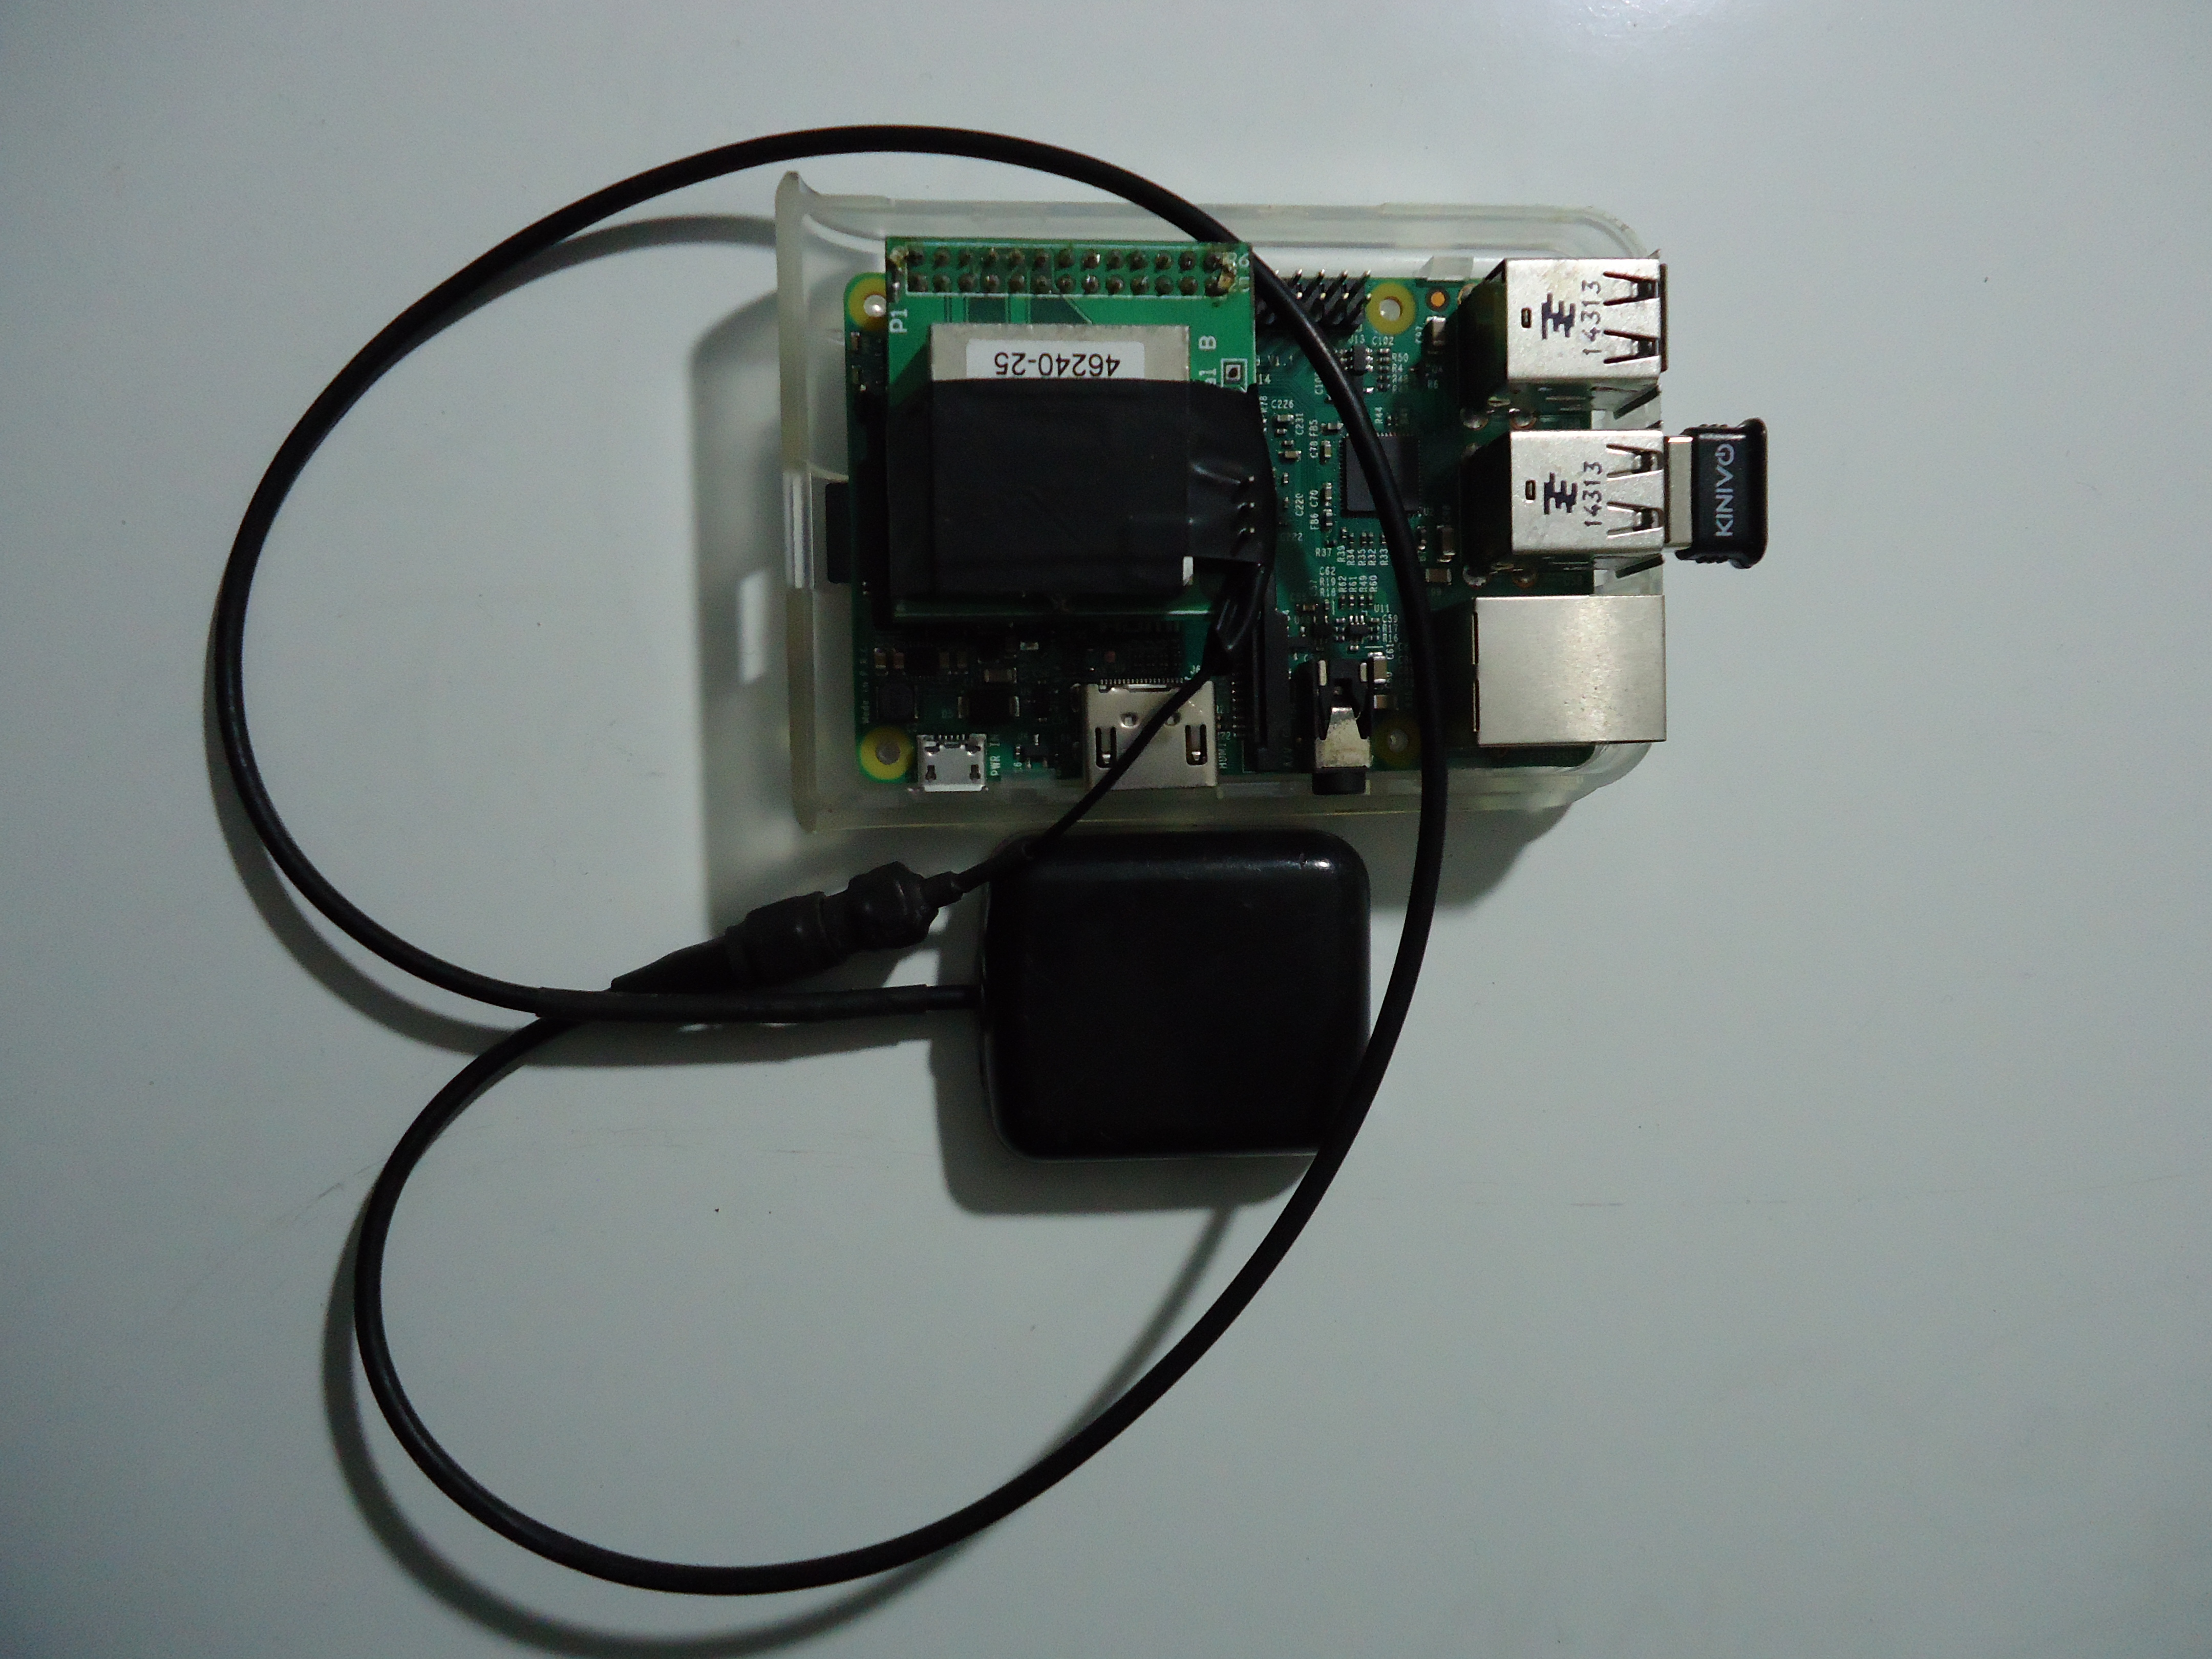
\includegraphics[width=0.45\textwidth]{../Pictures/v3/WCXI2015/DSC01916.JPG}
    \caption{Raspberry Pi B 2.0 with team-made GPS module}
\end{figure}

\begin{figure}[H]
    \centering
    \includegraphics[width=0.45\textwidth]{../Pictures/v3/WCXI2015/11402892_850967411605320_3887305866160117339_o.jpg}
    \caption{Winter Challenge XI (São Paulo, Brazil), 2015}
\end{figure}


\section{Past achievements} \label{past-achievements}
Our robot is one of the national favourites and proudly the international
third place. Being a reasonably recent project, it hasn't gone through a lot of
competitions. Following is a list of past achievents.

\subsection*{2014}
\setcounter{subsubsection}{0}
\subsubsection{Winter Challenge X} Third place
\subsection*{2015}
\setcounter{subsubsection}{0}
\subsubsection{RoboGames 2015} Third place
\subsubsection{Winter Challenge XI} Fifth place




\section{Sponsorship}


\section*{Acknowledgment}


\begin{thebibliography}{99}
    \bibitem{ThundeRatz}
    Thunderatz Robotics Team. http://thunderatz.org/
    \bibitem{RoboCore}
    RoboCore. \emph{Sua tecnologia à prova}. https://www.robocore.net/
    \bibitem{SRS}
    Seattle Robotics Society. \emph{SRS Robo-Magellan}. http://www.robothon.org/robothon/robo-magellan.php
    \bibitem{Campus-Future}
    Campus Party. \emph{Campus Future}. http://brasil.campus-party.org/conteudos/open-campus/campus-future/
    \bibitem{exemplo} Ator 1, Ator 2, \textit{Publicação}. link
\end{thebibliography}

Falar sobre patrocínio Trekking!

\end{document}

% An example of a floating figure using the graphicx package.
% Note that \label must occur AFTER (or within) \caption.
% For figures, \caption should occur after the \includegraphics.
% Note that IEEEtran v1.7 and later has special internal code that
% is designed to preserve the operation of \label within \caption
% even when the captionsoff option is in effect. However, because
% of issues like this, it may be the safest practice to put all your
% \label just after \caption rather than within \caption{}.
%
% Reminder: the "draftcls" or "draftclsnofoot", not "draft", class
% option should be used if it is desired that the figures are to be
% displayed while in draft mode.
%
%\begin{figure}[!t]
%\centering
%\includegraphics[width=2.5in]{myfigure}
% where an .eps filename suffix will be assumed under latex,
% and a .pdf suffix will be assumed for pdflatex; or what has been declared
% via \DeclareGraphicsExtensions.
%\caption{Simulation results for the network.}
%\label{fig_sim}
%\end{figure}

% Note that IEEE typically puts floats only at the top, even when this
% results in a large percentage of a column being occupied by floats.


% An example of a double column floating figure using two subfigures.
% (The subfig.sty package must be loaded for this to work.)
% The subfigure \label commands are set within each subfloat command,
% and the \label for the overall figure must come after \caption.
% \hfil is used as a separator to get equal spacing.
% Watch out that the combined width of all the subfigures on a
% line do not exceed the text width or a line break will occur.
%
%\begin{figure*}[!t]
%\centering
%\subfloat[Case I]{\includegraphics[width=2.5in]{box}%
%\label{fig_first_case}}
%\hfil
%\subfloat[Case II]{\includegraphics[width=2.5in]{box}%
%\label{fig_second_case}}
%\caption{Simulation results for the network.}
%\label{fig_sim}
%\end{figure*}
%
% Note that often IEEE papers with subfigures do not employ subfigure
% captions (using the optional argument to \subfloat[]), but instead will
% reference/describe all of them (a), (b), etc., within the main caption.
% Be aware that for subfig.sty to generate the (a), (b), etc., subfigure
% labels, the optional argument to \subfloat must be present. If a
% subcaption is not desired, just leave its contents blank,
% e.g., \subfloat[].


% An example of a floating table. Note that, for IEEE style tables, the
% \caption command should come BEFORE the table and, given that table
% captions serve much like titles, are usually capitalized except for words
% such as a, an, and, as, at, but, by, for, in, nor, of, on, or, the, to
% and up, which are usually not capitalized unless they are the first or
% last word of the caption. Table text will default to \footnotesize as
% IEEE normally uses this smaller font for tables.
% The \label must come after \caption as always.
%
%\begin{table}[!t]
%% increase table row spacing, adjust to taste
%\renewcommand{\arraystretch}{1.3}
% if using array.sty, it might be a good idea to tweak the value of
% \extrarowheight as needed to properly center the text within the cells
%\caption{An Example of a Table}
%\label{table_example}
%\centering
%% Some packages, such as MDW tools, offer better commands for making tables
%% than the plain LaTeX2e tabular which is used here.
%\begin{tabular}{|c||c|}
%\hline
%One & Two\\
%\hline
%Three & Four\\
%\hline
%\end{tabular}
%\end{table}


% Note that the IEEE does not put floats in the very first column
% - or typically anywhere on the first page for that matter. Also,
% in-text middle ("here") positioning is typically not used, but it
% is allowed and encouraged for Computer Society conferences (but
% not Computer Society journals). Most IEEE journals/conferences use
% top floats exclusively.
% Note that, LaTeX2e, unlike IEEE journals/conferences, places
% footnotes above bottom floats. This can be corrected via the
% \fnbelowfloat command of the stfloats package.
